\documentclass[1p]{elsarticle_modified}
%\bibliographystyle{elsarticle-num}

%\usepackage[colorlinks]{hyperref}
%\usepackage{abbrmath_seonhwa} %\Abb, \Ascr, \Acal ,\Abf, \Afrak
\usepackage{amsfonts}
\usepackage{amssymb}
\usepackage{amsmath}
\usepackage{amsthm}
\usepackage{scalefnt}
\usepackage{amsbsy}
\usepackage{kotex}
\usepackage{caption}
\usepackage{subfig}
\usepackage{color}
\usepackage{graphicx}
\usepackage{xcolor} %% white, black, red, green, blue, cyan, magenta, yellow
\usepackage{float}
\usepackage{setspace}
\usepackage{hyperref}

\usepackage{tikz}
\usetikzlibrary{arrows}

\usepackage{multirow}
\usepackage{array} % fixed length table
\usepackage{hhline}

%%%%%%%%%%%%%%%%%%%%%
\makeatletter
\renewcommand*\env@matrix[1][\arraystretch]{%
	\edef\arraystretch{#1}%
	\hskip -\arraycolsep
	\let\@ifnextchar\new@ifnextchar
	\array{*\c@MaxMatrixCols c}}
\makeatother %https://tex.stackexchange.com/questions/14071/how-can-i-increase-the-line-spacing-in-a-matrix
%%%%%%%%%%%%%%%

\usepackage[normalem]{ulem}

\newcommand{\msout}[1]{\ifmmode\text{\sout{\ensuremath{#1}}}\else\sout{#1}\fi}
%SOURCE: \msout is \stkout macro in https://tex.stackexchange.com/questions/20609/strikeout-in-math-mode

\newcommand{\cancel}[1]{
	\ifmmode
	{\color{red}\msout{#1}}
	\else
	{\color{red}\sout{#1}}
	\fi
}

\newcommand{\add}[1]{
	{\color{blue}\uwave{#1}}
}

\newcommand{\replace}[2]{
	\ifmmode
	{\color{red}\msout{#1}}{\color{blue}\uwave{#2}}
	\else
	{\color{red}\sout{#1}}{\color{blue}\uwave{#2}}
	\fi
}

\newcommand{\Sol}{\mathcal{S}} %segment
\newcommand{\D}{D} %diagram
\newcommand{\A}{\mathcal{A}} %arc


%%%%%%%%%%%%%%%%%%%%%%%%%%%%%5 test

\def\sl{\operatorname{\textup{SL}}(2,\Cbb)}
\def\psl{\operatorname{\textup{PSL}}(2,\Cbb)}
\def\quan{\mkern 1mu \triangleright \mkern 1mu}

\theoremstyle{definition}
\newtheorem{thm}{Theorem}[section]
\newtheorem{prop}[thm]{Proposition}
\newtheorem{lem}[thm]{Lemma}
\newtheorem{ques}[thm]{Question}
\newtheorem{cor}[thm]{Corollary}
\newtheorem{defn}[thm]{Definition}
\newtheorem{exam}[thm]{Example}
\newtheorem{rmk}[thm]{Remark}
\newtheorem{alg}[thm]{Algorithm}

\newcommand{\I}{\sqrt{-1}}
\begin{document}

%\begin{frontmatter}
%
%\title{Boundary parabolic representations of knots up to 8 crossings}
%
%%% Group authors per affiliation:
%\author{Yunhi Cho} 
%\address{Department of Mathematics, University of Seoul, Seoul, Korea}
%\ead{yhcho@uos.ac.kr}
%
%
%\author{Seonhwa Kim} %\fnref{s_kim}}
%\address{Center for Geometry and Physics, Institute for Basic Science, Pohang, 37673, Korea}
%\ead{ryeona17@ibs.re.kr}
%
%\author{Hyuk Kim}
%\address{Department of Mathematical Sciences, Seoul National University, Seoul 08826, Korea}
%\ead{hyukkim@snu.ac.kr}
%
%\author{Seokbeom Yoon}
%\address{Department of Mathematical Sciences, Seoul National University, Seoul, 08826,  Korea}
%\ead{sbyoon15@snu.ac.kr}
%
%\begin{abstract}
%We find all boundary parabolic representation of knots up to 8 crossings.
%
%\end{abstract}
%\begin{keyword}
%    \MSC[2010] 57M25 
%\end{keyword}
%
%\end{frontmatter}

%\linenumbers
%\tableofcontents
%
\newcommand\colored[1]{\textcolor{white}{\rule[-0.35ex]{0.8em}{1.4ex}}\kern-0.8em\color{red} #1}%
%\newcommand\colored[1]{\textcolor{white}{ #1}\kern-2.17ex	\textcolor{white}{ #1}\kern-1.81ex	\textcolor{white}{ #1}\kern-2.15ex\color{red}#1	}

{\Large $\underline{12n_{0253}~(K12n_{0253})}$}

\setlength{\tabcolsep}{10pt}
\renewcommand{\arraystretch}{1.6}
\vspace{1cm}\begin{tabular}{m{100pt}>{\centering\arraybackslash}m{274pt}}
\multirow{5}{120pt}{
	\centering
	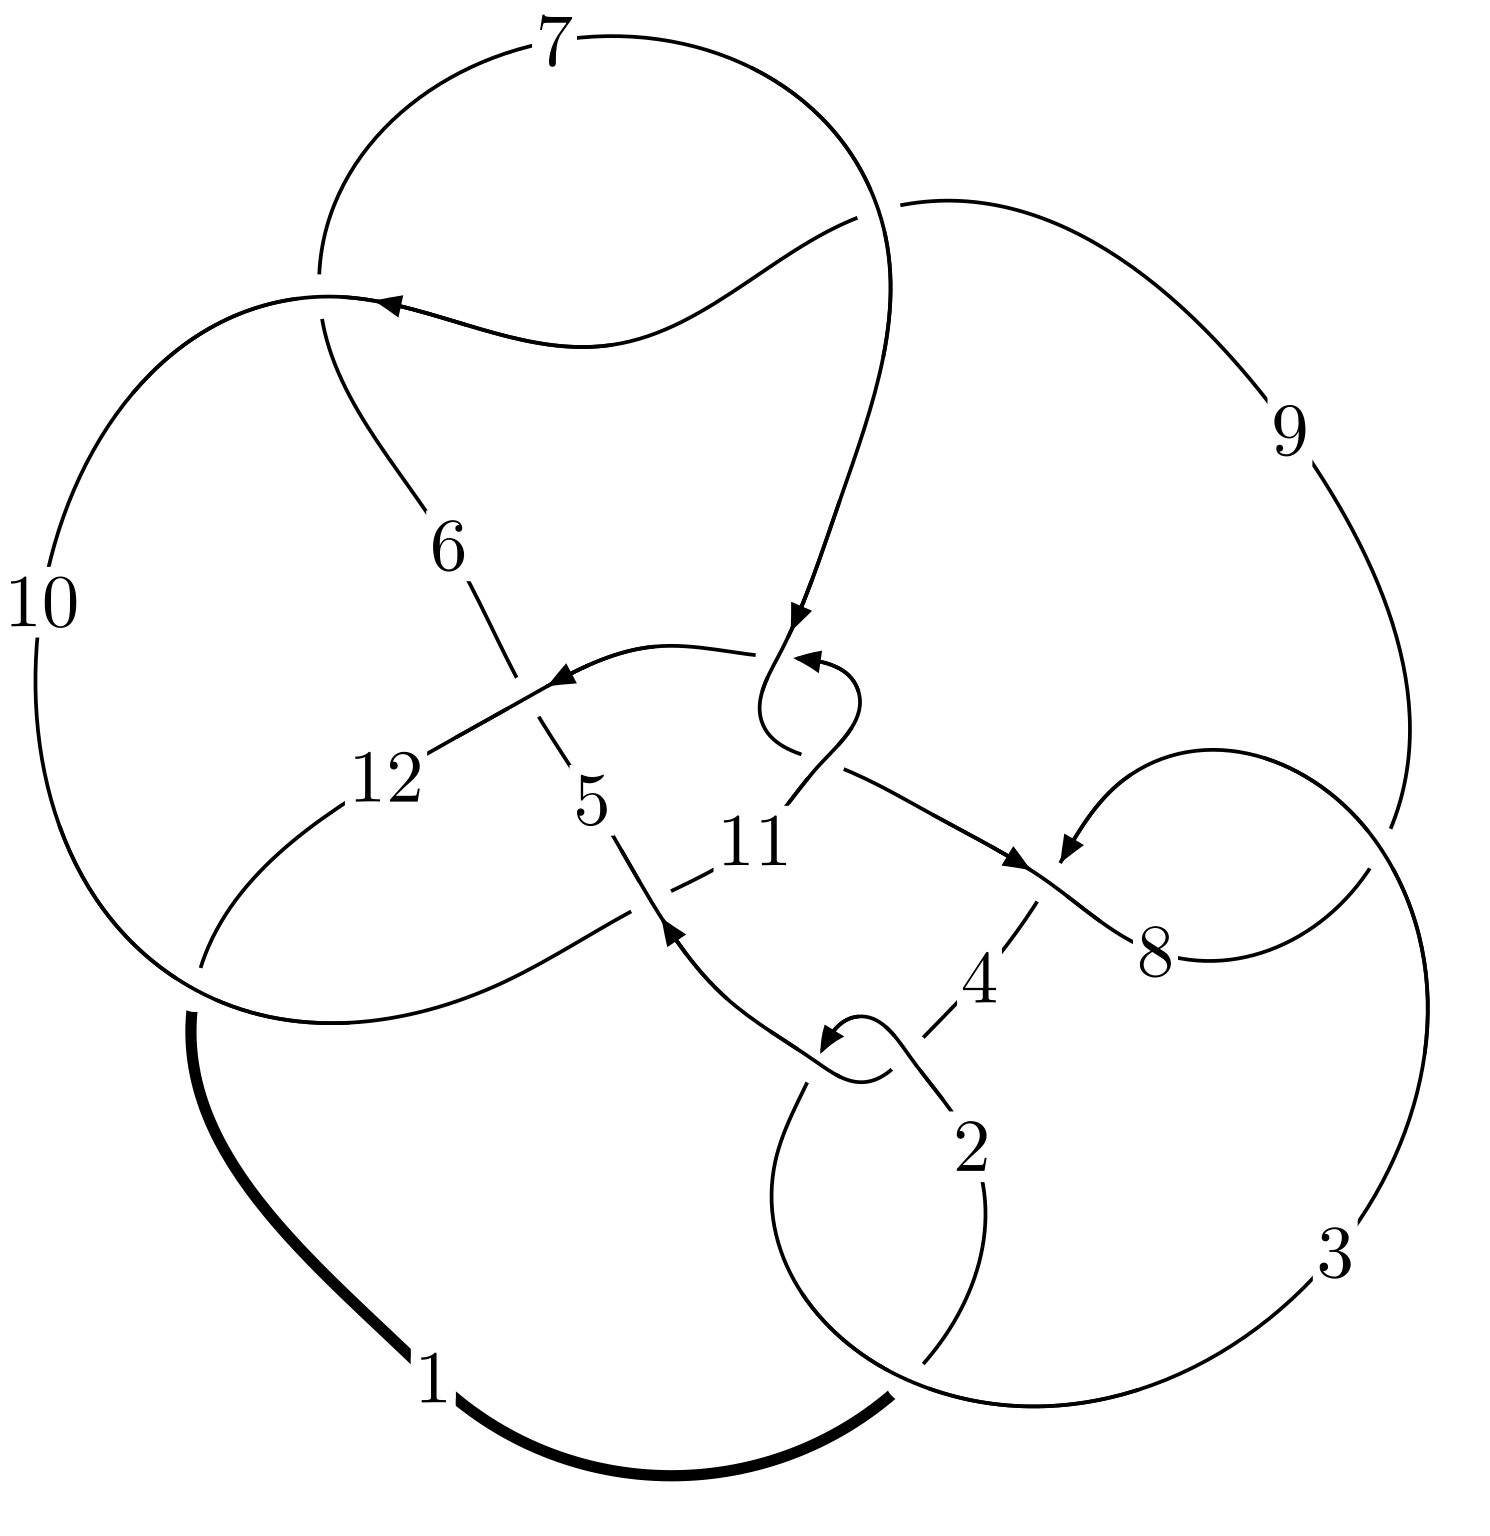
\includegraphics[width=112pt]{../../../GIT/diagram.site/Diagrams/png/2342_12n_0253.png}\\
\ \ \ A knot diagram\footnotemark}&
\allowdisplaybreaks
\textbf{Linearized knot diagam} \\
\cline{2-2}
 &
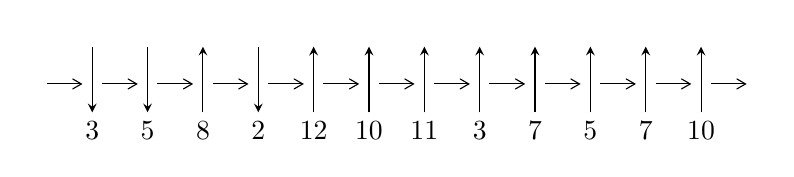
\begin{tikzpicture}[x=20pt, y=17pt]
	% nodes
	\node (C0) at (0, 0) {};
	\node (C1) at (1, 0) {};
	\node (C1U) at (1, +1) {};
	\node (C1D) at (1, -1) {3};

	\node (C2) at (2, 0) {};
	\node (C2U) at (2, +1) {};
	\node (C2D) at (2, -1) {5};

	\node (C3) at (3, 0) {};
	\node (C3U) at (3, +1) {};
	\node (C3D) at (3, -1) {8};

	\node (C4) at (4, 0) {};
	\node (C4U) at (4, +1) {};
	\node (C4D) at (4, -1) {2};

	\node (C5) at (5, 0) {};
	\node (C5U) at (5, +1) {};
	\node (C5D) at (5, -1) {12};

	\node (C6) at (6, 0) {};
	\node (C6U) at (6, +1) {};
	\node (C6D) at (6, -1) {10};

	\node (C7) at (7, 0) {};
	\node (C7U) at (7, +1) {};
	\node (C7D) at (7, -1) {11};

	\node (C8) at (8, 0) {};
	\node (C8U) at (8, +1) {};
	\node (C8D) at (8, -1) {3};

	\node (C9) at (9, 0) {};
	\node (C9U) at (9, +1) {};
	\node (C9D) at (9, -1) {7};

	\node (C10) at (10, 0) {};
	\node (C10U) at (10, +1) {};
	\node (C10D) at (10, -1) {5};

	\node (C11) at (11, 0) {};
	\node (C11U) at (11, +1) {};
	\node (C11D) at (11, -1) {7};

	\node (C12) at (12, 0) {};
	\node (C12U) at (12, +1) {};
	\node (C12D) at (12, -1) {10};
	\node (C13) at (13, 0) {};

	% arrows
	\draw[->,>={angle 60}]
	(C0) edge (C1) (C1) edge (C2) (C2) edge (C3) (C3) edge (C4) (C4) edge (C5) (C5) edge (C6) (C6) edge (C7) (C7) edge (C8) (C8) edge (C9) (C9) edge (C10) (C10) edge (C11) (C11) edge (C12) (C12) edge (C13) ;	\draw[->,>=stealth]
	(C1U) edge (C1D) (C2U) edge (C2D) (C3D) edge (C3U) (C4U) edge (C4D) (C5D) edge (C5U) (C6D) edge (C6U) (C7D) edge (C7U) (C8D) edge (C8U) (C9D) edge (C9U) (C10D) edge (C10U) (C11D) edge (C11U) (C12D) edge (C12U) ;
	\end{tikzpicture} \\
\hhline{~~} \\& 
\textbf{Solving Sequence} \\ \cline{2-2} 
 &
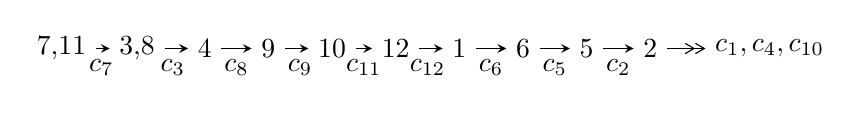
\begin{tikzpicture}[x=23pt, y=7pt]
	% node
	\node (A0) at (-1/8, 0) {7,11};
	\node (A1) at (17/16, 0) {3,8};
	\node (A2) at (17/8, 0) {4};
	\node (A3) at (25/8, 0) {9};
	\node (A4) at (33/8, 0) {10};
	\node (A5) at (41/8, 0) {12};
	\node (A6) at (49/8, 0) {1};
	\node (A7) at (57/8, 0) {6};
	\node (A8) at (65/8, 0) {5};
	\node (A9) at (73/8, 0) {2};
	\node (C1) at (1/2, -1) {$c_{7}$};
	\node (C2) at (13/8, -1) {$c_{3}$};
	\node (C3) at (21/8, -1) {$c_{8}$};
	\node (C4) at (29/8, -1) {$c_{9}$};
	\node (C5) at (37/8, -1) {$c_{11}$};
	\node (C6) at (45/8, -1) {$c_{12}$};
	\node (C7) at (53/8, -1) {$c_{6}$};
	\node (C8) at (61/8, -1) {$c_{5}$};
	\node (C9) at (69/8, -1) {$c_{2}$};
	\node (A10) at (11, 0) {$c_{1},c_{4},c_{10}$};

	% edge
	\draw[->,>=stealth]	
	(A0) edge (A1) (A1) edge (A2) (A2) edge (A3) (A3) edge (A4) (A4) edge (A5) (A5) edge (A6) (A6) edge (A7) (A7) edge (A8) (A8) edge (A9) ;
	\draw[->>,>={angle 60}]	
	(A9) edge (A10);
\end{tikzpicture} \\ 

\end{tabular} \\

\footnotetext{
The image of knot diagram is generated by the software ``\textbf{Draw programme}" developed by Andrew Bartholomew(\url{http://www.layer8.co.uk/maths/draw/index.htm\#Running-draw}), where we modified some parts for our purpose(\url{https://github.com/CATsTAILs/LinksPainter}).
}\phantom \\ \newline 
\centering \textbf{Ideals for irreducible components\footnotemark of $X_{\text{par}}$} 
 
\begin{align*}
I^u_{1}&=\langle 
7195073323 u^{17}-14120105470 u^{16}+\cdots+28350336356 b+9967888544,\\
\phantom{I^u_{1}}&\phantom{= \langle  }10882383441 u^{17}-7621235445 u^{16}+\cdots+28350336356 a-6834662691,\;u^{18}- u^{17}+\cdots+2 u-1\rangle \\
I^u_{2}&=\langle 
u^3+b+1,\;- u^2+a- u-1,\;u^4+u^3+2 u^2+2 u+1\rangle \\
I^u_{3}&=\langle 
3.21010\times10^{22} u^{19}+1.39979\times10^{23} u^{18}+\cdots+1.27572\times10^{24} b-1.65660\times10^{24},\\
\phantom{I^u_{3}}&\phantom{= \langle  }4.70076\times10^{24} u^{19}+1.58931\times10^{25} u^{18}+\cdots+1.28848\times10^{26} a-8.29304\times10^{26},\\
\phantom{I^u_{3}}&\phantom{= \langle  }u^{20}+3 u^{19}+\cdots-376 u-101\rangle \\
I^u_{4}&=\langle 
- u^4- u^2+b-2 u-2,\;2 u^4- u^3+3 u^2+a+4 u+2,\;u^5- u^4+u^3+2 u^2- u-1\rangle \\
I^u_{5}&=\langle 
2 b+1,\;2 a+u-2,\;u^2- u-1\rangle \\
\\
\end{align*}
\raggedright * 5 irreducible components of $\dim_{\mathbb{C}}=0$, with total 49 representations.\\
\footnotetext{All coefficients of polynomials are rational numbers. But the coefficients are sometimes approximated in decimal forms when there is not enough margin.}
\newpage
\renewcommand{\arraystretch}{1}
\centering \section*{I. $I^u_{1}= \langle 7.20\times10^{9} u^{17}-1.41\times10^{10} u^{16}+\cdots+2.84\times10^{10} b+9.97\times10^{9},\;1.09\times10^{10} u^{17}-7.62\times10^{9} u^{16}+\cdots+2.84\times10^{10} a-6.83\times10^{9},\;u^{18}- u^{17}+\cdots+2 u-1 \rangle$}
\flushleft \textbf{(i) Arc colorings}\\
\begin{tabular}{m{7pt} m{180pt} m{7pt} m{180pt} }
\flushright $a_{7}=$&$\begin{pmatrix}1\\0\end{pmatrix}$ \\
\flushright $a_{11}=$&$\begin{pmatrix}0\\u\end{pmatrix}$ \\
\flushright $a_{3}=$&$\begin{pmatrix}-0.383854 u^{17}+0.268823 u^{16}+\cdots+8.54749 u+0.241079\\-0.253791 u^{17}+0.498058 u^{16}+\cdots+0.630885 u-0.351597\end{pmatrix}$ \\
\flushright $a_{8}=$&$\begin{pmatrix}1\\- u^2\end{pmatrix}$ \\
\flushright $a_{4}=$&$\begin{pmatrix}-0.777946 u^{17}+0.831176 u^{16}+\cdots+9.02458 u-0.225548\\-0.526419 u^{17}+0.757093 u^{16}+\cdots+1.36150 u-0.519857\end{pmatrix}$ \\
\flushright $a_{9}=$&$\begin{pmatrix}-0.397400 u^{17}+0.367268 u^{16}+\cdots+0.173895 u-0.480447\\0.397400 u^{17}-0.367268 u^{16}+\cdots-1.17390 u+0.480447\end{pmatrix}$ \\
\flushright $a_{10}=$&$\begin{pmatrix}- u\\0.397400 u^{17}-0.367268 u^{16}+\cdots-1.17390 u+0.480447\end{pmatrix}$ \\
\flushright $a_{12}=$&$\begin{pmatrix}u\\u\end{pmatrix}$ \\
\flushright $a_{1}=$&$\begin{pmatrix}-0.0564932 u^{17}+0.000418696 u^{16}+\cdots+1.33714 u+0.0301320\\0.397400 u^{17}-0.367268 u^{16}+\cdots-1.17390 u+0.480447\end{pmatrix}$ \\
\flushright $a_{6}=$&$\begin{pmatrix}-0.0301320 u^{17}+0.0866252 u^{16}+\cdots+0.314353 u+0.602600\\-0.510579 u^{17}+0.169672 u^{16}+\cdots+1.32635 u+0.815602\end{pmatrix}$ \\
\flushright $a_{5}=$&$\begin{pmatrix}1\\-0.480447 u^{17}+0.0830471 u^{16}+\cdots+1.01199 u+1.21300\end{pmatrix}$ \\
\flushright $a_{2}=$&$\begin{pmatrix}-0.0850210 u^{17}-0.406163 u^{16}+\cdots+4.28732 u+2.74100\\0.642918 u^{17}-0.279464 u^{16}+\cdots-1.90934 u-0.721817\end{pmatrix}$\\&\end{tabular}
\flushleft \textbf{(ii) Obstruction class $= -1$}\\~\\
\flushleft \textbf{(iii) Cusp Shapes $= \frac{48478562013}{14175168178} u^{17}-\frac{74014314443}{56700672712} u^{16}+\cdots-\frac{808636576713}{56700672712} u-\frac{444360496187}{56700672712}$}\\~\\
\newpage\renewcommand{\arraystretch}{1}
\flushleft \textbf{(iv) u-Polynomials at the component}\newline \\
\begin{tabular}{m{50pt}|m{274pt}}
Crossings & \hspace{64pt}u-Polynomials at each crossing \\
\hline $$\begin{aligned}c_{1}\end{aligned}$$&$\begin{aligned}
&u^{18}+17 u^{17}+\cdots+9840 u+256
\end{aligned}$\\
\hline $$\begin{aligned}c_{2},c_{4}\end{aligned}$$&$\begin{aligned}
&u^{18}-3 u^{17}+\cdots-108 u+16
\end{aligned}$\\
\hline $$\begin{aligned}c_{3},c_{8}\end{aligned}$$&$\begin{aligned}
&u^{18}+5 u^{17}+\cdots-144 u+64
\end{aligned}$\\
\hline $$\begin{aligned}c_{5},c_{6},c_{9}\end{aligned}$$&$\begin{aligned}
&u^{18}-10 u^{16}+\cdots+3 u+1
\end{aligned}$\\
\hline $$\begin{aligned}c_{7},c_{10},c_{11}\end{aligned}$$&$\begin{aligned}
&u^{18}+u^{17}+\cdots-2 u-1
\end{aligned}$\\
\hline $$\begin{aligned}c_{12}\end{aligned}$$&$\begin{aligned}
&u^{18}+19 u^{17}+\cdots-352 u-32
\end{aligned}$\\
\hline
\end{tabular}\\~\\
\newpage\renewcommand{\arraystretch}{1}
\flushleft \textbf{(v) Riley Polynomials at the component}\newline \\
\begin{tabular}{m{50pt}|m{274pt}}
Crossings & \hspace{64pt}Riley Polynomials at each crossing \\
\hline $$\begin{aligned}c_{1}\end{aligned}$$&$\begin{aligned}
&y^{18}-29 y^{17}+\cdots-79539968 y+65536
\end{aligned}$\\
\hline $$\begin{aligned}c_{2},c_{4}\end{aligned}$$&$\begin{aligned}
&y^{18}-17 y^{17}+\cdots-9840 y+256
\end{aligned}$\\
\hline $$\begin{aligned}c_{3},c_{8}\end{aligned}$$&$\begin{aligned}
&y^{18}+9 y^{17}+\cdots-45824 y+4096
\end{aligned}$\\
\hline $$\begin{aligned}c_{5},c_{6},c_{9}\end{aligned}$$&$\begin{aligned}
&y^{18}-20 y^{17}+\cdots-13 y+1
\end{aligned}$\\
\hline $$\begin{aligned}c_{7},c_{10},c_{11}\end{aligned}$$&$\begin{aligned}
&y^{18}+17 y^{17}+\cdots+22 y+1
\end{aligned}$\\
\hline $$\begin{aligned}c_{12}\end{aligned}$$&$\begin{aligned}
&y^{18}-7 y^{17}+\cdots+2560 y+1024
\end{aligned}$\\
\hline
\end{tabular}\\~\\
\newpage\flushleft \textbf{(vi) Complex Volumes and Cusp Shapes}
$$\begin{array}{c|c|c}  
\text{Solutions to }I^u_{1}& \I (\text{vol} + \sqrt{-1}CS) & \text{Cusp shape}\\
 \hline 
\begin{aligned}
u &= \phantom{-}0.118044 + 0.790449 I \\
a &= \phantom{-}0.241077 - 0.719892 I \\
b &= -1.304910 - 0.071727 I\end{aligned}
 & \phantom{-}3.00375 + 0.37123 I & \phantom{-}4.92078 - 0.99425 I \\ \hline\begin{aligned}
u &= \phantom{-}0.118044 - 0.790449 I \\
a &= \phantom{-}0.241077 + 0.719892 I \\
b &= -1.304910 + 0.071727 I\end{aligned}
 & \phantom{-}3.00375 - 0.37123 I & \phantom{-}4.92078 + 0.99425 I \\ \hline\begin{aligned}
u &= -0.065288 + 1.324970 I \\
a &= -0.241397 + 1.248350 I \\
b &= -0.138781 + 0.489222 I\end{aligned}
 & -2.87372 - 1.22079 I & \phantom{-}4.21569 + 1.79625 I \\ \hline\begin{aligned}
u &= -0.065288 - 1.324970 I \\
a &= -0.241397 - 1.248350 I \\
b &= -0.138781 - 0.489222 I\end{aligned}
 & -2.87372 + 1.22079 I & \phantom{-}4.21569 - 1.79625 I \\ \hline\begin{aligned}
u &= \phantom{-}0.077894 + 0.510339 I \\
a &= -0.365385 + 1.013810 I \\
b &= \phantom{-}1.153220 - 0.268641 I\end{aligned}
 & \phantom{-}1.16211 - 5.14367 I & \phantom{-}0.72332 + 8.80281 I \\ \hline\begin{aligned}
u &= \phantom{-}0.077894 - 0.510339 I \\
a &= -0.365385 - 1.013810 I \\
b &= \phantom{-}1.153220 + 0.268641 I\end{aligned}
 & \phantom{-}1.16211 + 5.14367 I & \phantom{-}0.72332 - 8.80281 I \\ \hline\begin{aligned}
u &= \phantom{-}0.29181 + 1.48433 I \\
a &= -0.145718 + 0.537802 I \\
b &= \phantom{-}1.77462 + 0.55736 I\end{aligned}
 & -4.07395 + 5.05034 I & \phantom{-}3.51840 - 3.93444 I \\ \hline\begin{aligned}
u &= \phantom{-}0.29181 - 1.48433 I \\
a &= -0.145718 - 0.537802 I \\
b &= \phantom{-}1.77462 - 0.55736 I\end{aligned}
 & -4.07395 - 5.05034 I & \phantom{-}3.51840 + 3.93444 I \\ \hline\begin{aligned}
u &= \phantom{-}0.82095 + 1.28564 I \\
a &= \phantom{-}0.739381 - 0.956915 I \\
b &= -0.835011 - 0.397109 I\end{aligned}
 & -13.28510 + 3.46125 I & \phantom{-}10.05857 - 2.89058 I \\ \hline\begin{aligned}
u &= \phantom{-}0.82095 - 1.28564 I \\
a &= \phantom{-}0.739381 + 0.956915 I \\
b &= -0.835011 + 0.397109 I\end{aligned}
 & -13.28510 - 3.46125 I & \phantom{-}10.05857 + 2.89058 I\\
 \hline 
 \end{array}$$\newpage$$\begin{array}{c|c|c}  
\text{Solutions to }I^u_{1}& \I (\text{vol} + \sqrt{-1}CS) & \text{Cusp shape}\\
 \hline 
\begin{aligned}
u &= \phantom{-}1.53352\phantom{ +0.000000I} \\
a &= \phantom{-}0.113874\phantom{ +0.000000I} \\
b &= -0.624141\phantom{ +0.000000I}\end{aligned}
 & \phantom{-}7.37422\phantom{ +0.000000I} & \phantom{-}37.5360\phantom{ +0.000000I} \\ \hline\begin{aligned}
u &= -0.465205\phantom{ +0.000000I} \\
a &= -0.483543\phantom{ +0.000000I} \\
b &= -0.301112\phantom{ +0.000000I}\end{aligned}
 & \phantom{-}0.706459\phantom{ +0.000000I} & \phantom{-}14.1730\phantom{ +0.000000I} \\ \hline\begin{aligned}
u &= -0.54788 + 1.47697 I \\
a &= -0.066154 - 1.204480 I \\
b &= \phantom{-}1.025710 - 0.899512 I\end{aligned}
 & -0.56915 - 8.13906 I & \phantom{-}5.11000 + 5.47218 I \\ \hline\begin{aligned}
u &= -0.54788 - 1.47697 I \\
a &= -0.066154 + 1.204480 I \\
b &= \phantom{-}1.025710 + 0.899512 I\end{aligned}
 & -0.56915 + 8.13906 I & \phantom{-}5.11000 - 5.47218 I \\ \hline\begin{aligned}
u &= \phantom{-}0.126997 + 0.287207 I \\
a &= \phantom{-}0.04063 + 2.28012 I \\
b &= \phantom{-}0.432312 - 0.429086 I\end{aligned}
 & -1.64243 + 0.66705 I & -2.34520 - 2.39491 I \\ \hline\begin{aligned}
u &= \phantom{-}0.126997 - 0.287207 I \\
a &= \phantom{-}0.04063 - 2.28012 I \\
b &= \phantom{-}0.432312 + 0.429086 I\end{aligned}
 & -1.64243 - 0.66705 I & -2.34520 + 2.39491 I \\ \hline\begin{aligned}
u &= -0.85668 + 1.69020 I \\
a &= \phantom{-}0.232404 + 1.080370 I \\
b &= -1.64453 + 1.59807 I\end{aligned}
 & -6.3235 - 13.9812 I & \phantom{-}2.81858 + 6.62298 I \\ \hline\begin{aligned}
u &= -0.85668 - 1.69020 I \\
a &= \phantom{-}0.232404 - 1.080370 I \\
b &= -1.64453 - 1.59807 I\end{aligned}
 & -6.3235 + 13.9812 I & \phantom{-}2.81858 - 6.62298 I\\
 \hline 
 \end{array}$$\newpage\newpage\renewcommand{\arraystretch}{1}
\centering \section*{II. $I^u_{2}= \langle u^3+b+1,\;- u^2+a- u-1,\;u^4+u^3+2 u^2+2 u+1 \rangle$}
\flushleft \textbf{(i) Arc colorings}\\
\begin{tabular}{m{7pt} m{180pt} m{7pt} m{180pt} }
\flushright $a_{7}=$&$\begin{pmatrix}1\\0\end{pmatrix}$ \\
\flushright $a_{11}=$&$\begin{pmatrix}0\\u\end{pmatrix}$ \\
\flushright $a_{3}=$&$\begin{pmatrix}u^2+u+1\\- u^3-1\end{pmatrix}$ \\
\flushright $a_{8}=$&$\begin{pmatrix}1\\- u^2\end{pmatrix}$ \\
\flushright $a_{4}=$&$\begin{pmatrix}- u^3- u-1\\- u^3- u-1\end{pmatrix}$ \\
\flushright $a_{9}=$&$\begin{pmatrix}u^3+u^2+u+2\\- u^3- u^2-2 u-2\end{pmatrix}$ \\
\flushright $a_{10}=$&$\begin{pmatrix}- u\\- u^3- u^2-2 u-2\end{pmatrix}$ \\
\flushright $a_{12}=$&$\begin{pmatrix}u\\u\end{pmatrix}$ \\
\flushright $a_{1}=$&$\begin{pmatrix}u^3+2 u\\u^3+u^2+2 u+2\end{pmatrix}$ \\
\flushright $a_{6}=$&$\begin{pmatrix}0\\2 u^3+u^2+3 u+2\end{pmatrix}$ \\
\flushright $a_{5}=$&$\begin{pmatrix}-1\\2 u^3+u^2+3 u+1\end{pmatrix}$ \\
\flushright $a_{2}=$&$\begin{pmatrix}u\\u^3+3 u+1\end{pmatrix}$\\&\end{tabular}
\flushleft \textbf{(ii) Obstruction class $= 1$}\\~\\
\flushleft \textbf{(iii) Cusp Shapes $= 5 u^2+u+8$}\\~\\
\newpage\renewcommand{\arraystretch}{1}
\flushleft \textbf{(iv) u-Polynomials at the component}\newline \\
\begin{tabular}{m{50pt}|m{274pt}}
Crossings & \hspace{64pt}u-Polynomials at each crossing \\
\hline $$\begin{aligned}c_{1}\end{aligned}$$&$\begin{aligned}
&u^4-3 u^3+5 u^2-3 u+1
\end{aligned}$\\
\hline $$\begin{aligned}c_{2}\end{aligned}$$&$\begin{aligned}
&u^4+u^3- u^2- u+1
\end{aligned}$\\
\hline $$\begin{aligned}c_{3},c_{5},c_{9}\end{aligned}$$&$\begin{aligned}
&u^4-2 u^3+2 u^2- u+1
\end{aligned}$\\
\hline $$\begin{aligned}c_{4},c_{12}\end{aligned}$$&$\begin{aligned}
&u^4- u^3- u^2+u+1
\end{aligned}$\\
\hline $$\begin{aligned}c_{6},c_{8}\end{aligned}$$&$\begin{aligned}
&u^4+2 u^3+2 u^2+u+1
\end{aligned}$\\
\hline $$\begin{aligned}c_{7},c_{10}\end{aligned}$$&$\begin{aligned}
&u^4+u^3+2 u^2+2 u+1
\end{aligned}$\\
\hline $$\begin{aligned}c_{11}\end{aligned}$$&$\begin{aligned}
&u^4- u^3+2 u^2-2 u+1
\end{aligned}$\\
\hline
\end{tabular}\\~\\
\newpage\renewcommand{\arraystretch}{1}
\flushleft \textbf{(v) Riley Polynomials at the component}\newline \\
\begin{tabular}{m{50pt}|m{274pt}}
Crossings & \hspace{64pt}Riley Polynomials at each crossing \\
\hline $$\begin{aligned}c_{1}\end{aligned}$$&$\begin{aligned}
&y^4+y^3+9 y^2+y+1
\end{aligned}$\\
\hline $$\begin{aligned}c_{2},c_{4},c_{12}\end{aligned}$$&$\begin{aligned}
&y^4-3 y^3+5 y^2-3 y+1
\end{aligned}$\\
\hline $$\begin{aligned}c_{3},c_{5},c_{6}\\c_{8},c_{9}\end{aligned}$$&$\begin{aligned}
&y^4+2 y^2+3 y+1
\end{aligned}$\\
\hline $$\begin{aligned}c_{7},c_{10},c_{11}\end{aligned}$$&$\begin{aligned}
&y^4+3 y^3+2 y^2+1
\end{aligned}$\\
\hline
\end{tabular}\\~\\
\newpage\flushleft \textbf{(vi) Complex Volumes and Cusp Shapes}
$$\begin{array}{c|c|c}  
\text{Solutions to }I^u_{2}& \I (\text{vol} + \sqrt{-1}CS) & \text{Cusp shape}\\
 \hline 
\begin{aligned}
u &= -0.621744 + 0.440597 I \\
a &= \phantom{-}0.570696 - 0.107280 I \\
b &= -1.121740 - 0.425428 I\end{aligned}
 & \phantom{-}1.74699 + 4.62527 I & \phantom{-}8.34046 - 2.29879 I \\ \hline\begin{aligned}
u &= -0.621744 - 0.440597 I \\
a &= \phantom{-}0.570696 + 0.107280 I \\
b &= -1.121740 + 0.425428 I\end{aligned}
 & \phantom{-}1.74699 - 4.62527 I & \phantom{-}8.34046 + 2.29879 I \\ \hline\begin{aligned}
u &= \phantom{-}0.121744 + 1.306620 I \\
a &= -0.57070 + 1.62477 I \\
b &= -0.37826 + 2.17265 I\end{aligned}
 & -5.03685 + 0.56550 I & -0.34046 + 2.89736 I \\ \hline\begin{aligned}
u &= \phantom{-}0.121744 - 1.306620 I \\
a &= -0.57070 - 1.62477 I \\
b &= -0.37826 - 2.17265 I\end{aligned}
 & -5.03685 - 0.56550 I & -0.34046 - 2.89736 I\\
 \hline 
 \end{array}$$\newpage\newpage\renewcommand{\arraystretch}{1}
\centering \section*{III. $I^u_{3}= \langle 3.21\times10^{22} u^{19}+1.40\times10^{23} u^{18}+\cdots+1.28\times10^{24} b-1.66\times10^{24},\;4.70\times10^{24} u^{19}+1.59\times10^{25} u^{18}+\cdots+1.29\times10^{26} a-8.29\times10^{26},\;u^{20}+3 u^{19}+\cdots-376 u-101 \rangle$}
\flushleft \textbf{(i) Arc colorings}\\
\begin{tabular}{m{7pt} m{180pt} m{7pt} m{180pt} }
\flushright $a_{7}=$&$\begin{pmatrix}1\\0\end{pmatrix}$ \\
\flushright $a_{11}=$&$\begin{pmatrix}0\\u\end{pmatrix}$ \\
\flushright $a_{3}=$&$\begin{pmatrix}-0.0364831 u^{19}-0.123348 u^{18}+\cdots-2.99222 u+6.43631\\-0.0251630 u^{19}-0.109726 u^{18}+\cdots+10.5249 u+1.29856\end{pmatrix}$ \\
\flushright $a_{8}=$&$\begin{pmatrix}1\\- u^2\end{pmatrix}$ \\
\flushright $a_{4}=$&$\begin{pmatrix}-0.0190479 u^{19}-0.0791729 u^{18}+\cdots-1.37806 u+6.33110\\0.00211539 u^{19}-0.0452946 u^{18}+\cdots+11.8210 u+2.11973\end{pmatrix}$ \\
\flushright $a_{9}=$&$\begin{pmatrix}-0.0344491 u^{19}-0.0902792 u^{18}+\cdots-0.756139 u+5.71229\\-0.0246550 u^{19}-0.0750446 u^{18}+\cdots+4.35620 u-0.000767038\end{pmatrix}$ \\
\flushright $a_{10}=$&$\begin{pmatrix}-0.0591041 u^{19}-0.165324 u^{18}+\cdots+3.60006 u+5.71152\\-0.0246550 u^{19}-0.0750446 u^{18}+\cdots+4.35620 u-0.000767038\end{pmatrix}$ \\
\flushright $a_{12}=$&$\begin{pmatrix}u\\u\end{pmatrix}$ \\
\flushright $a_{1}=$&$\begin{pmatrix}0.0699474 u^{19}+0.209299 u^{18}+\cdots-4.79549 u-9.53973\\0.0255973 u^{19}+0.0893164 u^{18}+\cdots-5.84866 u-0.104669\end{pmatrix}$ \\
\flushright $a_{6}=$&$\begin{pmatrix}-0.0266289 u^{19}-0.0263605 u^{18}+\cdots-1.12655 u-5.56497\\-0.0255925 u^{19}-0.0488488 u^{18}+\cdots-2.27935 u-0.105970\end{pmatrix}$ \\
\flushright $a_{5}=$&$\begin{pmatrix}-0.0141044 u^{19}-0.0539607 u^{18}+\cdots+8.39337 u-2.97964\\-0.0130681 u^{19}-0.0764490 u^{18}+\cdots+7.24057 u+2.47936\end{pmatrix}$ \\
\flushright $a_{2}=$&$\begin{pmatrix}0.00280493 u^{19}-0.0244296 u^{18}+\cdots+1.75093 u+2.31489\\-0.0326545 u^{19}-0.134709 u^{18}+\cdots+10.6296 u+2.01431\end{pmatrix}$\\&\end{tabular}
\flushleft \textbf{(ii) Obstruction class $= -1$}\\~\\
\flushleft \textbf{(iii) Cusp Shapes $= \frac{1916248316412301273576}{20913445507764897101425} u^{19}+\frac{6077402466516369822264}{20913445507764897101425} u^{18}+\cdots-\frac{339832460854605717393908}{20913445507764897101425} u+\frac{38632741605919100523346}{20913445507764897101425}$}\\~\\
\newpage\renewcommand{\arraystretch}{1}
\flushleft \textbf{(iv) u-Polynomials at the component}\newline \\
\begin{tabular}{m{50pt}|m{274pt}}
Crossings & \hspace{64pt}u-Polynomials at each crossing \\
\hline $$\begin{aligned}c_{1}\end{aligned}$$&$\begin{aligned}
&(u^5+5 u^4+8 u^3+3 u^2- u+1)^4
\end{aligned}$\\
\hline $$\begin{aligned}c_{2},c_{4}\end{aligned}$$&$\begin{aligned}
&(u^5- u^4-2 u^3+u^2+u+1)^4
\end{aligned}$\\
\hline $$\begin{aligned}c_{3},c_{8}\end{aligned}$$&$\begin{aligned}
&(u^5- u^4+2 u^3- u^2+u-1)^4
\end{aligned}$\\
\hline $$\begin{aligned}c_{5},c_{6},c_{9}\end{aligned}$$&$\begin{aligned}
&u^{20}+3 u^{19}+\cdots-690 u-209
\end{aligned}$\\
\hline $$\begin{aligned}c_{7},c_{10},c_{11}\end{aligned}$$&$\begin{aligned}
&u^{20}-3 u^{19}+\cdots+376 u-101
\end{aligned}$\\
\hline $$\begin{aligned}c_{12}\end{aligned}$$&$\begin{aligned}
&(u^2- u-1)^{10}
\end{aligned}$\\
\hline
\end{tabular}\\~\\
\newpage\renewcommand{\arraystretch}{1}
\flushleft \textbf{(v) Riley Polynomials at the component}\newline \\
\begin{tabular}{m{50pt}|m{274pt}}
Crossings & \hspace{64pt}Riley Polynomials at each crossing \\
\hline $$\begin{aligned}c_{1}\end{aligned}$$&$\begin{aligned}
&(y^5-9 y^4+32 y^3-35 y^2-5 y-1)^4
\end{aligned}$\\
\hline $$\begin{aligned}c_{2},c_{4}\end{aligned}$$&$\begin{aligned}
&(y^5-5 y^4+8 y^3-3 y^2- y-1)^4
\end{aligned}$\\
\hline $$\begin{aligned}c_{3},c_{8}\end{aligned}$$&$\begin{aligned}
&(y^5+3 y^4+4 y^3+y^2- y-1)^4
\end{aligned}$\\
\hline $$\begin{aligned}c_{5},c_{6},c_{9}\end{aligned}$$&$\begin{aligned}
&y^{20}-9 y^{19}+\cdots-194368 y+43681
\end{aligned}$\\
\hline $$\begin{aligned}c_{7},c_{10},c_{11}\end{aligned}$$&$\begin{aligned}
&y^{20}+11 y^{19}+\cdots-147436 y+10201
\end{aligned}$\\
\hline $$\begin{aligned}c_{12}\end{aligned}$$&$\begin{aligned}
&(y^2-3 y+1)^{10}
\end{aligned}$\\
\hline
\end{tabular}\\~\\
\newpage\flushleft \textbf{(vi) Complex Volumes and Cusp Shapes}
$$\begin{array}{c|c|c}  
\text{Solutions to }I^u_{3}& \I (\text{vol} + \sqrt{-1}CS) & \text{Cusp shape}\\
 \hline 
\begin{aligned}
u &= \phantom{-}1.18182\phantom{ +0.000000I} \\
a &= -3.08950\phantom{ +0.000000I} \\
b &= \phantom{-}3.54825\phantom{ +0.000000I}\end{aligned}
 & \phantom{-}1.54676\phantom{ +0.000000I} & \phantom{-}4.51890\phantom{ +0.000000I} \\ \hline\begin{aligned}
u &= \phantom{-}0.392602 + 1.119800 I \\
a &= \phantom{-}0.865506 - 0.649555 I \\
b &= \phantom{-}0.719869 - 0.653025 I\end{aligned}
 & -4.27694 + 1.53058 I & \phantom{-}5.48489 - 4.43065 I \\ \hline\begin{aligned}
u &= \phantom{-}0.392602 - 1.119800 I \\
a &= \phantom{-}0.865506 + 0.649555 I \\
b &= \phantom{-}0.719869 + 0.653025 I\end{aligned}
 & -4.27694 - 1.53058 I & \phantom{-}5.48489 + 4.43065 I \\ \hline\begin{aligned}
u &= -1.251030 + 0.315505 I \\
a &= -0.411298 + 0.093081 I \\
b &= \phantom{-}0.868398 + 0.361281 I\end{aligned}
 & \phantom{-}3.61874 + 1.53058 I & \phantom{-}5.48489 - 4.43065 I \\ \hline\begin{aligned}
u &= -1.251030 - 0.315505 I \\
a &= -0.411298 - 0.093081 I \\
b &= \phantom{-}0.868398 - 0.361281 I\end{aligned}
 & \phantom{-}3.61874 - 1.53058 I & \phantom{-}5.48489 + 4.43065 I \\ \hline\begin{aligned}
u &= \phantom{-}0.342814 + 0.586956 I \\
a &= -1.19319 - 3.16782 I \\
b &= -1.206580 + 0.583471 I\end{aligned}
 & \phantom{-}3.61874 + 1.53058 I & \phantom{-}5.48489 - 4.43065 I \\ \hline\begin{aligned}
u &= \phantom{-}0.342814 - 0.586956 I \\
a &= -1.19319 + 3.16782 I \\
b &= -1.206580 - 0.583471 I\end{aligned}
 & \phantom{-}3.61874 - 1.53058 I & \phantom{-}5.48489 + 4.43065 I \\ \hline\begin{aligned}
u &= -0.181709 + 1.389530 I \\
a &= -1.37865 - 0.57028 I \\
b &= -3.09521 - 1.77844 I\end{aligned}
 & -6.34892\phantom{ +0.000000I} & \phantom{-}4.51886 + 0. I\phantom{ +0.000000I} \\ \hline\begin{aligned}
u &= -0.181709 - 1.389530 I \\
a &= -1.37865 + 0.57028 I \\
b &= -3.09521 + 1.77844 I\end{aligned}
 & -6.34892\phantom{ +0.000000I} & \phantom{-}4.51886 + 0. I\phantom{ +0.000000I} \\ \hline\begin{aligned}
u &= -0.11218 + 1.41123 I \\
a &= \phantom{-}0.578243 + 0.977323 I \\
b &= \phantom{-}0.379194 + 0.917038 I\end{aligned}
 & -1.92472 + 4.40083 I & \phantom{-}1.25569 - 3.49859 I\\
 \hline 
 \end{array}$$\newpage$$\begin{array}{c|c|c}  
\text{Solutions to }I^u_{3}& \I (\text{vol} + \sqrt{-1}CS) & \text{Cusp shape}\\
 \hline 
\begin{aligned}
u &= -0.11218 - 1.41123 I \\
a &= \phantom{-}0.578243 - 0.977323 I \\
b &= \phantom{-}0.379194 - 0.917038 I\end{aligned}
 & -1.92472 - 4.40083 I & \phantom{-}1.25569 + 3.49859 I \\ \hline\begin{aligned}
u &= -0.04570 + 1.46451 I \\
a &= -0.003969 + 1.233620 I \\
b &= \phantom{-}0.16549 + 1.82037 I\end{aligned}
 & -4.27694 - 1.53058 I & \phantom{-}5.48489 + 4.43065 I \\ \hline\begin{aligned}
u &= -0.04570 - 1.46451 I \\
a &= -0.003969 - 1.233620 I \\
b &= \phantom{-}0.16549 - 1.82037 I\end{aligned}
 & -4.27694 + 1.53058 I & \phantom{-}5.48489 - 4.43065 I \\ \hline\begin{aligned}
u &= \phantom{-}1.15161 + 1.24448 I \\
a &= -0.402882 + 0.473976 I \\
b &= \phantom{-}0.813208 + 0.060105 I\end{aligned}
 & -9.82040 + 4.40083 I & \phantom{-}1.25569 - 3.49859 I \\ \hline\begin{aligned}
u &= \phantom{-}1.15161 - 1.24448 I \\
a &= -0.402882 - 0.473976 I \\
b &= \phantom{-}0.813208 - 0.060105 I\end{aligned}
 & -9.82040 - 4.40083 I & \phantom{-}1.25569 + 3.49859 I \\ \hline\begin{aligned}
u &= -0.230378\phantom{ +0.000000I} \\
a &= \phantom{-}7.85497\phantom{ +0.000000I} \\
b &= -1.18372\phantom{ +0.000000I}\end{aligned}
 & \phantom{-}1.54676\phantom{ +0.000000I} & \phantom{-}4.51890\phantom{ +0.000000I} \\ \hline\begin{aligned}
u &= -1.88238 + 0.35860 I \\
a &= \phantom{-}0.067918 + 0.167881 I \\
b &= -0.91426 - 1.68174 I\end{aligned}
 & -1.92472 + 4.40083 I & \phantom{-}1.25569 - 3.49859 I \\ \hline\begin{aligned}
u &= -1.88238 - 0.35860 I \\
a &= \phantom{-}0.067918 - 0.167881 I \\
b &= -0.91426 + 1.68174 I\end{aligned}
 & -1.92472 - 4.40083 I & \phantom{-}1.25569 + 3.49859 I \\ \hline\begin{aligned}
u &= -0.38975 + 1.92049 I \\
a &= -0.068772 - 0.859380 I \\
b &= \phantom{-}0.58762 - 1.94190 I\end{aligned}
 & -9.82040 - 4.40083 I & \phantom{-}1.25569 + 3.49859 I \\ \hline\begin{aligned}
u &= -0.38975 - 1.92049 I \\
a &= -0.068772 + 0.859380 I \\
b &= \phantom{-}0.58762 + 1.94190 I\end{aligned}
 & -9.82040 + 4.40083 I & \phantom{-}1.25569 - 3.49859 I\\
 \hline 
 \end{array}$$\newpage\newpage\renewcommand{\arraystretch}{1}
\centering \section*{IV. $I^u_{4}= \langle - u^4- u^2+b-2 u-2,\;2 u^4- u^3+3 u^2+a+4 u+2,\;u^5- u^4+u^3+2 u^2- u-1 \rangle$}
\flushleft \textbf{(i) Arc colorings}\\
\begin{tabular}{m{7pt} m{180pt} m{7pt} m{180pt} }
\flushright $a_{7}=$&$\begin{pmatrix}1\\0\end{pmatrix}$ \\
\flushright $a_{11}=$&$\begin{pmatrix}0\\u\end{pmatrix}$ \\
\flushright $a_{3}=$&$\begin{pmatrix}-2 u^4+u^3-3 u^2-4 u-2\\u^4+u^2+2 u+2\end{pmatrix}$ \\
\flushright $a_{8}=$&$\begin{pmatrix}1\\- u^2\end{pmatrix}$ \\
\flushright $a_{4}=$&$\begin{pmatrix}-3 u^4+2 u^3-4 u^2-5 u-1\\u^4- u^3+u^2+3 u+2\end{pmatrix}$ \\
\flushright $a_{9}=$&$\begin{pmatrix}- u^4+u^3- u^2-3 u+1\\u^4- u^3+u^2+2 u-1\end{pmatrix}$ \\
\flushright $a_{10}=$&$\begin{pmatrix}- u\\u^4- u^3+u^2+2 u-1\end{pmatrix}$ \\
\flushright $a_{12}=$&$\begin{pmatrix}u\\u\end{pmatrix}$ \\
\flushright $a_{1}=$&$\begin{pmatrix}u^3+2 u\\- u^4+u^3- u^2-2 u+1\end{pmatrix}$ \\
\flushright $a_{6}=$&$\begin{pmatrix}0\\- u^4+2 u^3-2 u^2- u+3\end{pmatrix}$ \\
\flushright $a_{5}=$&$\begin{pmatrix}-1\\- u^4+2 u^3-2 u^2- u+2\end{pmatrix}$ \\
\flushright $a_{2}=$&$\begin{pmatrix}- u^4- u^2-3 u-3\\2 u^3- u^2+u+3\end{pmatrix}$\\&\end{tabular}
\flushleft \textbf{(ii) Obstruction class $= 1$}\\~\\
\flushleft \textbf{(iii) Cusp Shapes $= 6 u^4+3 u^3+5 u^2+16 u+19$}\\~\\
\newpage\renewcommand{\arraystretch}{1}
\flushleft \textbf{(iv) u-Polynomials at the component}\newline \\
\begin{tabular}{m{50pt}|m{274pt}}
Crossings & \hspace{64pt}u-Polynomials at each crossing \\
\hline $$\begin{aligned}c_{1}\end{aligned}$$&$\begin{aligned}
&u^5-7 u^4+15 u^3-7 u^2-2 u-1
\end{aligned}$\\
\hline $$\begin{aligned}c_{2}\end{aligned}$$&$\begin{aligned}
&u^5+3 u^4+u^3-3 u^2-2 u-1
\end{aligned}$\\
\hline $$\begin{aligned}c_{3}\end{aligned}$$&$\begin{aligned}
&u^5+2 u^4+5 u^3+4 u^2-1
\end{aligned}$\\
\hline $$\begin{aligned}c_{4}\end{aligned}$$&$\begin{aligned}
&u^5-3 u^4+u^3+3 u^2-2 u+1
\end{aligned}$\\
\hline $$\begin{aligned}c_{5},c_{9}\end{aligned}$$&$\begin{aligned}
&u^5- u^4-2 u^3+u^2+u+1
\end{aligned}$\\
\hline $$\begin{aligned}c_{6}\end{aligned}$$&$\begin{aligned}
&u^5+u^4-2 u^3- u^2+u-1
\end{aligned}$\\
\hline $$\begin{aligned}c_{7},c_{10}\end{aligned}$$&$\begin{aligned}
&u^5- u^4+u^3+2 u^2- u-1
\end{aligned}$\\
\hline $$\begin{aligned}c_{8}\end{aligned}$$&$\begin{aligned}
&u^5-2 u^4+5 u^3-4 u^2+1
\end{aligned}$\\
\hline $$\begin{aligned}c_{11}\end{aligned}$$&$\begin{aligned}
&u^5+u^4+u^3-2 u^2- u+1
\end{aligned}$\\
\hline $$\begin{aligned}c_{12}\end{aligned}$$&$\begin{aligned}
&u^5-4 u^4+9 u^3-21 u^2+31 u-17
\end{aligned}$\\
\hline
\end{tabular}\\~\\
\newpage\renewcommand{\arraystretch}{1}
\flushleft \textbf{(v) Riley Polynomials at the component}\newline \\
\begin{tabular}{m{50pt}|m{274pt}}
Crossings & \hspace{64pt}Riley Polynomials at each crossing \\
\hline $$\begin{aligned}c_{1}\end{aligned}$$&$\begin{aligned}
&y^5-19 y^4+123 y^3-123 y^2-10 y-1
\end{aligned}$\\
\hline $$\begin{aligned}c_{2},c_{4}\end{aligned}$$&$\begin{aligned}
&y^5-7 y^4+15 y^3-7 y^2-2 y-1
\end{aligned}$\\
\hline $$\begin{aligned}c_{3},c_{8}\end{aligned}$$&$\begin{aligned}
&y^5+6 y^4+9 y^3-12 y^2+8 y-1
\end{aligned}$\\
\hline $$\begin{aligned}c_{5},c_{6},c_{9}\end{aligned}$$&$\begin{aligned}
&y^5-5 y^4+8 y^3-3 y^2- y-1
\end{aligned}$\\
\hline $$\begin{aligned}c_{7},c_{10},c_{11}\end{aligned}$$&$\begin{aligned}
&y^5+y^4+3 y^3-8 y^2+5 y-1
\end{aligned}$\\
\hline $$\begin{aligned}c_{12}\end{aligned}$$&$\begin{aligned}
&y^5+2 y^4-25 y^3-19 y^2+247 y-289
\end{aligned}$\\
\hline
\end{tabular}\\~\\
\newpage\flushleft \textbf{(vi) Complex Volumes and Cusp Shapes}
$$\begin{array}{c|c|c}  
\text{Solutions to }I^u_{4}& \I (\text{vol} + \sqrt{-1}CS) & \text{Cusp shape}\\
 \hline 
\begin{aligned}
u &= \phantom{-}0.821196\phantom{ +0.000000I} \\
a &= -7.66362\phantom{ +0.000000I} \\
b &= \phantom{-}4.77152\phantom{ +0.000000I}\end{aligned}
 & \phantom{-}2.16633\phantom{ +0.000000I} & \phantom{-}39.9010\phantom{ +0.000000I} \\ \hline\begin{aligned}
u &= -0.688402 + 0.106340 I \\
a &= -1.322140 + 0.434760 I \\
b &= \phantom{-}1.278340 - 0.069185 I\end{aligned}
 & \phantom{-}4.53993 + 0.30358 I & \phantom{-}10.54519 + 0.60661 I \\ \hline\begin{aligned}
u &= -0.688402 - 0.106340 I \\
a &= -1.322140 - 0.434760 I \\
b &= \phantom{-}1.278340 + 0.069185 I\end{aligned}
 & \phantom{-}4.53993 - 0.30358 I & \phantom{-}10.54519 - 0.60661 I \\ \hline\begin{aligned}
u &= \phantom{-}0.77780 + 1.38013 I \\
a &= \phantom{-}0.653954 - 0.923165 I \\
b &= -0.664098 - 0.673862 I\end{aligned}
 & -13.8478 + 3.3875 I & -4.49564 - 1.04146 I \\ \hline\begin{aligned}
u &= \phantom{-}0.77780 - 1.38013 I \\
a &= \phantom{-}0.653954 + 0.923165 I \\
b &= -0.664098 + 0.673862 I\end{aligned}
 & -13.8478 - 3.3875 I & -4.49564 + 1.04146 I\\
 \hline 
 \end{array}$$\newpage\newpage\renewcommand{\arraystretch}{1}
\centering \section*{V. $I^u_{5}= \langle 2 b+1,\;2 a+u-2,\;u^2- u-1 \rangle$}
\flushleft \textbf{(i) Arc colorings}\\
\begin{tabular}{m{7pt} m{180pt} m{7pt} m{180pt} }
\flushright $a_{7}=$&$\begin{pmatrix}1\\0\end{pmatrix}$ \\
\flushright $a_{11}=$&$\begin{pmatrix}0\\u\end{pmatrix}$ \\
\flushright $a_{3}=$&$\begin{pmatrix}-\frac{1}{2} u+1\\-0.5\end{pmatrix}$ \\
\flushright $a_{8}=$&$\begin{pmatrix}1\\- u-1\end{pmatrix}$ \\
\flushright $a_{4}=$&$\begin{pmatrix}-\frac{1}{2} u+1\\-0.5\end{pmatrix}$ \\
\flushright $a_{9}=$&$\begin{pmatrix}1\\- u-1\end{pmatrix}$ \\
\flushright $a_{10}=$&$\begin{pmatrix}- u\\- u-1\end{pmatrix}$ \\
\flushright $a_{12}=$&$\begin{pmatrix}u\\u\end{pmatrix}$ \\
\flushright $a_{1}=$&$\begin{pmatrix}-1\\- u-1\end{pmatrix}$ \\
\flushright $a_{6}=$&$\begin{pmatrix}2 u+2\\3 u+2\end{pmatrix}$ \\
\flushright $a_{5}=$&$\begin{pmatrix}1\\u+1\end{pmatrix}$ \\
\flushright $a_{2}=$&$\begin{pmatrix}-\frac{1}{2} u\\- u-\frac{3}{2}\end{pmatrix}$\\&\end{tabular}
\flushleft \textbf{(ii) Obstruction class $= 1$}\\~\\
\flushleft \textbf{(iii) Cusp Shapes $= -\frac{45}{4} u-\frac{13}{4}$}\\~\\
\newpage\renewcommand{\arraystretch}{1}
\flushleft \textbf{(iv) u-Polynomials at the component}\newline \\
\begin{tabular}{m{50pt}|m{274pt}}
Crossings & \hspace{64pt}u-Polynomials at each crossing \\
\hline $$\begin{aligned}c_{1},c_{2}\end{aligned}$$&$\begin{aligned}
&(u-1)^2
\end{aligned}$\\
\hline $$\begin{aligned}c_{3},c_{8}\end{aligned}$$&$\begin{aligned}
&u^2
\end{aligned}$\\
\hline $$\begin{aligned}c_{4}\end{aligned}$$&$\begin{aligned}
&(u+1)^2
\end{aligned}$\\
\hline $$\begin{aligned}c_{5},c_{6}\end{aligned}$$&$\begin{aligned}
&u^2+3 u+1
\end{aligned}$\\
\hline $$\begin{aligned}c_{7}\end{aligned}$$&$\begin{aligned}
&u^2- u-1
\end{aligned}$\\
\hline $$\begin{aligned}c_{9}\end{aligned}$$&$\begin{aligned}
&u^2-3 u+1
\end{aligned}$\\
\hline $$\begin{aligned}c_{10},c_{11},c_{12}\end{aligned}$$&$\begin{aligned}
&u^2+u-1
\end{aligned}$\\
\hline
\end{tabular}\\~\\
\newpage\renewcommand{\arraystretch}{1}
\flushleft \textbf{(v) Riley Polynomials at the component}\newline \\
\begin{tabular}{m{50pt}|m{274pt}}
Crossings & \hspace{64pt}Riley Polynomials at each crossing \\
\hline $$\begin{aligned}c_{1},c_{2},c_{4}\end{aligned}$$&$\begin{aligned}
&(y-1)^2
\end{aligned}$\\
\hline $$\begin{aligned}c_{3},c_{8}\end{aligned}$$&$\begin{aligned}
&y^2
\end{aligned}$\\
\hline $$\begin{aligned}c_{5},c_{6},c_{9}\end{aligned}$$&$\begin{aligned}
&y^2-7 y+1
\end{aligned}$\\
\hline $$\begin{aligned}c_{7},c_{10},c_{11}\\c_{12}\end{aligned}$$&$\begin{aligned}
&y^2-3 y+1
\end{aligned}$\\
\hline
\end{tabular}\\~\\
\newpage\flushleft \textbf{(vi) Complex Volumes and Cusp Shapes}
$$\begin{array}{c|c|c}  
\text{Solutions to }I^u_{5}& \I (\text{vol} + \sqrt{-1}CS) & \text{Cusp shape}\\
 \hline 
\begin{aligned}
u &= -0.618034\phantom{ +0.000000I} \\
a &= \phantom{-}1.30902\phantom{ +0.000000I} \\
b &= -0.500000\phantom{ +0.000000I}\end{aligned}
 & -0.657974\phantom{ +0.000000I} & \phantom{-}3.70290\phantom{ +0.000000I} \\ \hline\begin{aligned}
u &= \phantom{-}1.61803\phantom{ +0.000000I} \\
a &= \phantom{-}0.190983\phantom{ +0.000000I} \\
b &= -0.500000\phantom{ +0.000000I}\end{aligned}
 & \phantom{-}7.23771\phantom{ +0.000000I} & -21.4530\phantom{ +0.000000I}\\
 \hline 
 \end{array}$$\newpage
\newpage\renewcommand{\arraystretch}{1}
\centering \section*{ VI. u-Polynomials}
\begin{tabular}{m{50pt}|m{274pt}}
Crossings & \hspace{64pt}u-Polynomials at each crossing \\
\hline $$\begin{aligned}c_{1}\end{aligned}$$&$\begin{aligned}
&(u-1)^2(u^4-3 u^3+5 u^2-3 u+1)(u^5-7 u^4+15 u^3-7 u^2-2 u-1)\\
&\cdot((u^5+5 u^4+8 u^3+3 u^2- u+1)^4)(u^{18}+17 u^{17}+\cdots+9840 u+256)
\end{aligned}$\\
\hline $$\begin{aligned}c_{2}\end{aligned}$$&$\begin{aligned}
&(u-1)^2(u^4+u^3- u^2- u+1)(u^5- u^4-2 u^3+u^2+u+1)^4\\
&\cdot(u^5+3 u^4+u^3-3 u^2-2 u-1)(u^{18}-3 u^{17}+\cdots-108 u+16)
\end{aligned}$\\
\hline $$\begin{aligned}c_{3}\end{aligned}$$&$\begin{aligned}
&u^2(u^4-2 u^3+2 u^2- u+1)(u^5- u^4+2 u^3- u^2+u-1)^4\\
&\cdot(u^5+2 u^4+5 u^3+4 u^2-1)(u^{18}+5 u^{17}+\cdots-144 u+64)
\end{aligned}$\\
\hline $$\begin{aligned}c_{4}\end{aligned}$$&$\begin{aligned}
&(u+1)^2(u^4- u^3- u^2+u+1)(u^5-3 u^4+u^3+3 u^2-2 u+1)\\
&\cdot((u^5- u^4-2 u^3+u^2+u+1)^4)(u^{18}-3 u^{17}+\cdots-108 u+16)
\end{aligned}$\\
\hline $$\begin{aligned}c_{5}\end{aligned}$$&$\begin{aligned}
&(u^2+3 u+1)(u^4-2 u^3+2 u^2- u+1)(u^5- u^4-2 u^3+u^2+u+1)\\
&\cdot(u^{18}-10 u^{16}+\cdots+3 u+1)(u^{20}+3 u^{19}+\cdots-690 u-209)
\end{aligned}$\\
\hline $$\begin{aligned}c_{6}\end{aligned}$$&$\begin{aligned}
&(u^2+3 u+1)(u^4+2 u^3+2 u^2+u+1)(u^5+u^4-2 u^3- u^2+u-1)\\
&\cdot(u^{18}-10 u^{16}+\cdots+3 u+1)(u^{20}+3 u^{19}+\cdots-690 u-209)
\end{aligned}$\\
\hline $$\begin{aligned}c_{7}\end{aligned}$$&$\begin{aligned}
&(u^2- u-1)(u^4+u^3+2 u^2+2 u+1)(u^5- u^4+u^3+2 u^2- u-1)\\
&\cdot(u^{18}+u^{17}+\cdots-2 u-1)(u^{20}-3 u^{19}+\cdots+376 u-101)
\end{aligned}$\\
\hline $$\begin{aligned}c_{8}\end{aligned}$$&$\begin{aligned}
&u^2(u^4+2 u^3+2 u^2+u+1)(u^5-2 u^4+5 u^3-4 u^2+1)\\
&\cdot((u^5- u^4+2 u^3- u^2+u-1)^4)(u^{18}+5 u^{17}+\cdots-144 u+64)
\end{aligned}$\\
\hline $$\begin{aligned}c_{9}\end{aligned}$$&$\begin{aligned}
&(u^2-3 u+1)(u^4-2 u^3+2 u^2- u+1)(u^5- u^4-2 u^3+u^2+u+1)\\
&\cdot(u^{18}-10 u^{16}+\cdots+3 u+1)(u^{20}+3 u^{19}+\cdots-690 u-209)
\end{aligned}$\\
\hline $$\begin{aligned}c_{10}\end{aligned}$$&$\begin{aligned}
&(u^2+u-1)(u^4+u^3+2 u^2+2 u+1)(u^5- u^4+u^3+2 u^2- u-1)\\
&\cdot(u^{18}+u^{17}+\cdots-2 u-1)(u^{20}-3 u^{19}+\cdots+376 u-101)
\end{aligned}$\\
\hline $$\begin{aligned}c_{11}\end{aligned}$$&$\begin{aligned}
&(u^2+u-1)(u^4- u^3+2 u^2-2 u+1)(u^5+u^4+u^3-2 u^2- u+1)\\
&\cdot(u^{18}+u^{17}+\cdots-2 u-1)(u^{20}-3 u^{19}+\cdots+376 u-101)
\end{aligned}$\\
\hline $$\begin{aligned}c_{12}\end{aligned}$$&$\begin{aligned}
&(u^2- u-1)^{10}(u^2+u-1)(u^4- u^3- u^2+u+1)\\
&\cdot(u^5-4 u^4+9 u^3-21 u^2+31 u-17)(u^{18}+19 u^{17}+\cdots-352 u-32)
\end{aligned}$\\
\hline
\end{tabular}\newpage\renewcommand{\arraystretch}{1}
\centering \section*{ VII. Riley Polynomials}
\begin{tabular}{m{50pt}|m{274pt}}
Crossings & \hspace{64pt}Riley Polynomials at each crossing \\
\hline $$\begin{aligned}c_{1}\end{aligned}$$&$\begin{aligned}
&((y-1)^2)(y^4+y^3+9 y^2+y+1)(y^5-19 y^4+\cdots-10 y-1)\\
&\cdot(y^5-9 y^4+32 y^3-35 y^2-5 y-1)^4\\
&\cdot(y^{18}-29 y^{17}+\cdots-79539968 y+65536)
\end{aligned}$\\
\hline $$\begin{aligned}c_{2},c_{4}\end{aligned}$$&$\begin{aligned}
&(y-1)^2(y^4-3 y^3+5 y^2-3 y+1)(y^5-7 y^4+15 y^3-7 y^2-2 y-1)\\
&\cdot((y^5-5 y^4+8 y^3-3 y^2- y-1)^4)(y^{18}-17 y^{17}+\cdots-9840 y+256)
\end{aligned}$\\
\hline $$\begin{aligned}c_{3},c_{8}\end{aligned}$$&$\begin{aligned}
&y^2(y^4+2 y^2+3 y+1)(y^5+3 y^4+4 y^3+y^2- y-1)^4\\
&\cdot(y^5+6 y^4+9 y^3-12 y^2+8 y-1)(y^{18}+9 y^{17}+\cdots-45824 y+4096)
\end{aligned}$\\
\hline $$\begin{aligned}c_{5},c_{6},c_{9}\end{aligned}$$&$\begin{aligned}
&(y^2-7 y+1)(y^4+2 y^2+3 y+1)(y^5-5 y^4+8 y^3-3 y^2- y-1)\\
&\cdot(y^{18}-20 y^{17}+\cdots-13 y+1)(y^{20}-9 y^{19}+\cdots-194368 y+43681)
\end{aligned}$\\
\hline $$\begin{aligned}c_{7},c_{10},c_{11}\end{aligned}$$&$\begin{aligned}
&(y^2-3 y+1)(y^4+3 y^3+2 y^2+1)(y^5+y^4+3 y^3-8 y^2+5 y-1)\\
&\cdot(y^{18}+17 y^{17}+\cdots+22 y+1)(y^{20}+11 y^{19}+\cdots-147436 y+10201)
\end{aligned}$\\
\hline $$\begin{aligned}c_{12}\end{aligned}$$&$\begin{aligned}
&(y^2-3 y+1)^{11}(y^4-3 y^3+5 y^2-3 y+1)\\
&\cdot(y^5+2 y^4-25 y^3-19 y^2+247 y-289)\\
&\cdot(y^{18}-7 y^{17}+\cdots+2560 y+1024)
\end{aligned}$\\
\hline
\end{tabular}
\vskip 2pc
\end{document}